\chapter{Experiments} \label{exp}

In our work we implemented two fusion neural networks:
\begin{itemize}
    \item simple network consisting of sequential convolutions on top of each scale; scheme of this network can be found of figure \ref{fig:fcn}; in table \ref{table:qual} with results we refer to this architecture as \textbf{FCN};
    \item UNet-like \cite{unet} architecture with downsampling and upsampling layers and residual connections; scheme of this network can be found on figure \ref{fig:unet}; in table \ref{table:qual} we refer to this architecture as \textbf{UNet}.
\end{itemize}

\begin{figure}
\caption{Fully convolutional network}
\centering
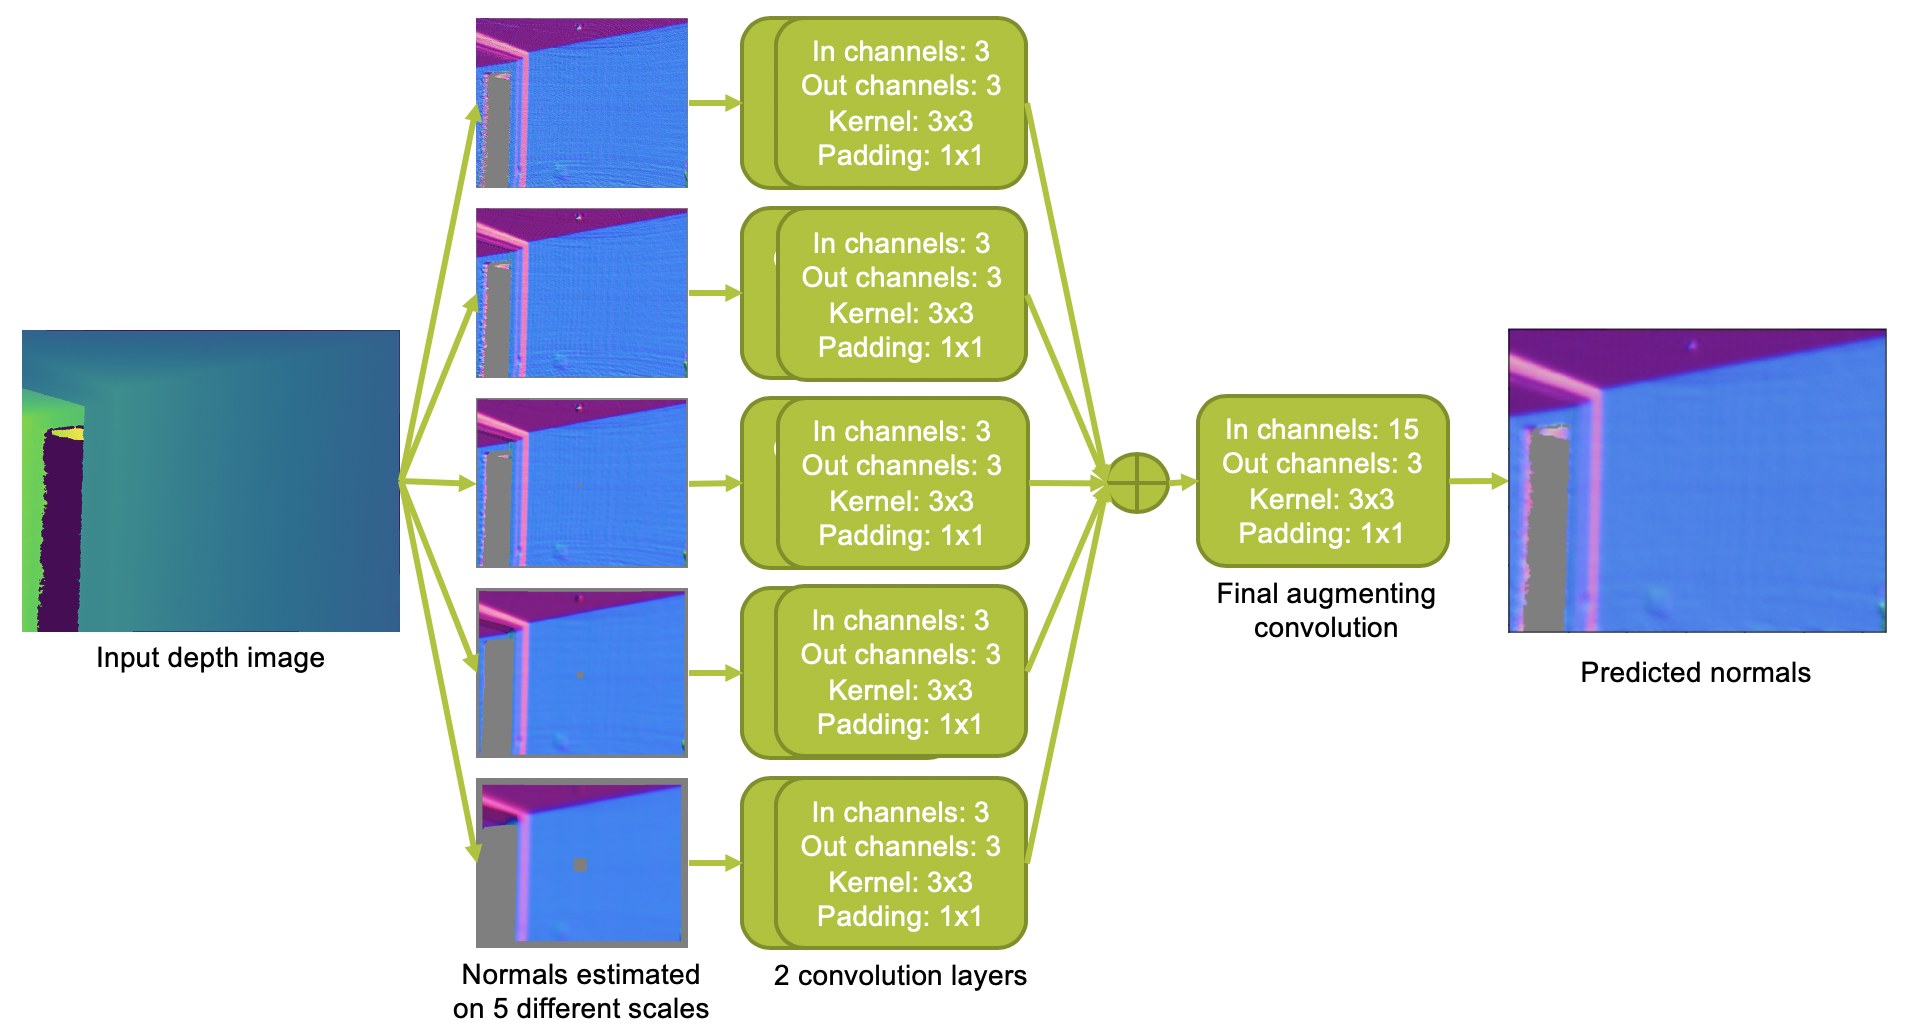
\includegraphics[width=\textwidth]{images/Screen Shot 2020-05-27 at 7.47.52 PM.png}
\label{fig:fcn}
\end{figure}

\begin{figure}
\caption{UNet-like convolutional network}
\centering
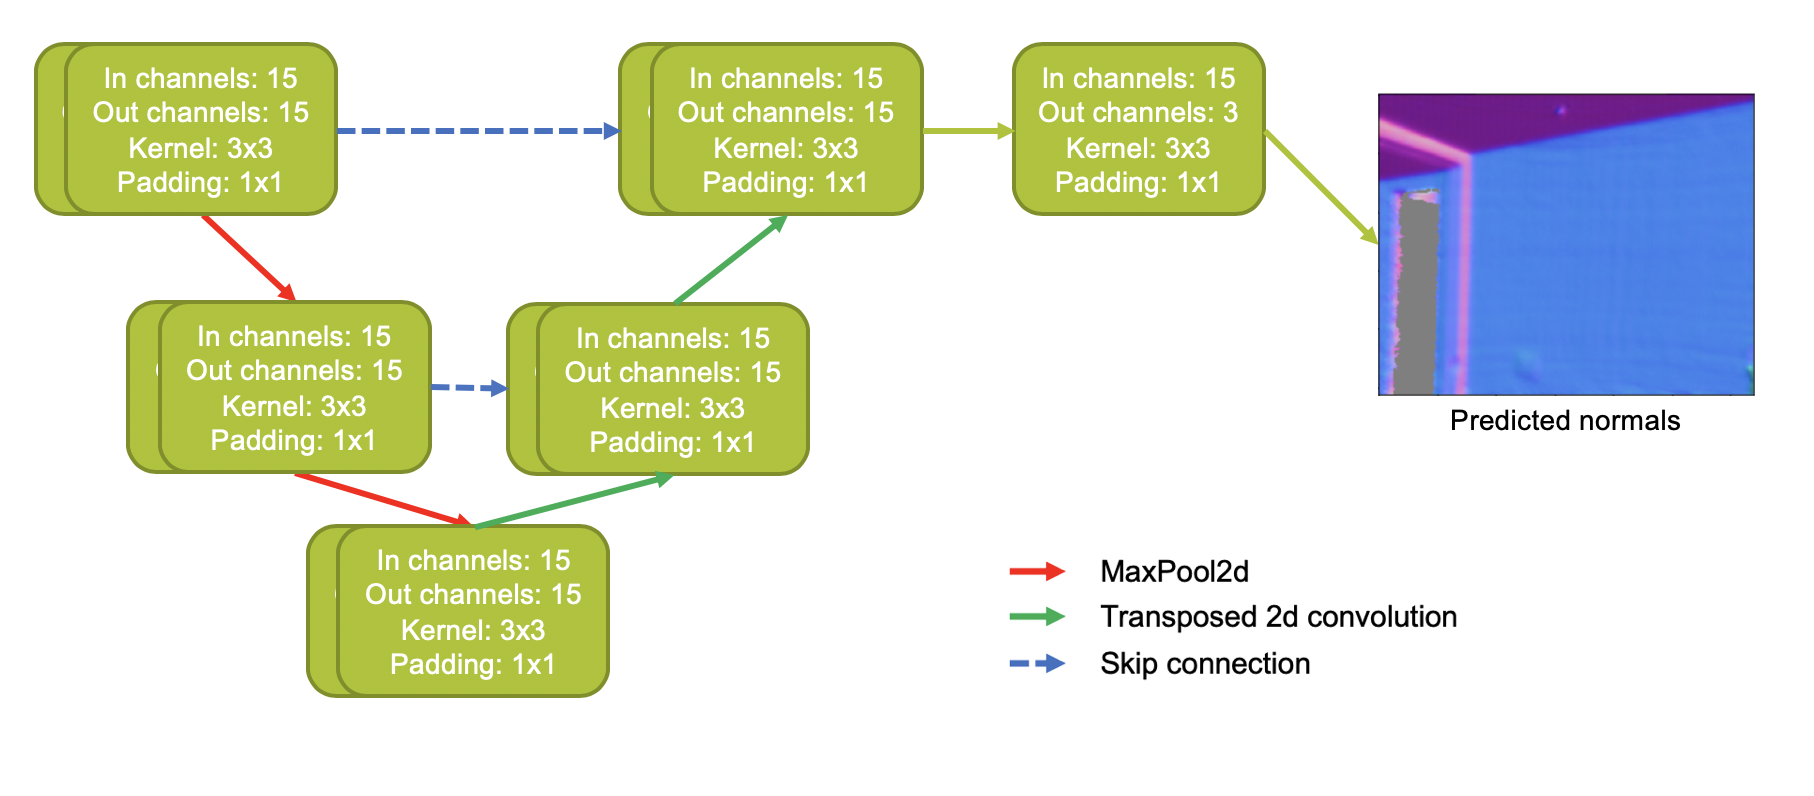
\includegraphics[width=\textwidth]{images/Screen Shot 2020-05-27 at 7.51.30 PM.png}
\label{fig:unet}
\end{figure}

We evaluated our algorithm on Matterport dataset comparing it with several depth-based and RGBD-based algorithm. For consistency we used same evaluation metrics as in other works \cite{deep_surf, deep_depth_compl}. They consist of:
\begin{itemize}
    \item mean angle distance in degrees between predicted and ground-truth normals;
    \item median angle distance between predicted and ground-truth normals;
    \item fraction of pixels where error is less than $11.25^{\circ}$;
    \item fraction of pixels where error is less than $22.5^{\circ}$;
    \item fraction of pixels where error is less than $30^{\circ}$.
\end{itemize}

Results can be found in table \ref{table:qual}. It is seen that our algorithm did not outperform state-of-the-art algorithm HFM \cite{deep_surf} while being quite close to it. We consider this a good result as soon as that approach uses both depth and color channels while we use only depth. Also results show that our algorithm outperformed other depth-based methods as well as open3d baseline.

\begin{table}
\centering
\begin{tabular}{ | c | c | c | c | c | c | c | c | }
\hline
 & \multicolumn{2}{|c|}{Depth based} & \multicolumn{2}{|c|}{RGBD based} & \multicolumn{2}{|c|}{\textbf{MsNE (Ours)}} & \\
 \hline
 & Levin's \cite{colorization-using-optimization} & DC \cite{deep_depth_compl} & GFMM \cite{guided-depth-enhancement} & HFM \cite{deep_surf} & \textbf{FCN} & \textbf{UNet} & Open3d \cite{open3d} \\
 \hline
 Mean & 21.588  & 19.126 & 16.537 & \textbf{13.062} & 15.54 & \textbf{15.11} & 20.94 \\  
 \hline
 Median & 12.079  & 9.563 & 8.028 & \textbf{6.090} & 8.40 & \textbf{8.31} & 13.66 \\  
 \hline
 $11.25^{\circ}$ & 58.07  & 64.89 & 65.3 & \textbf{72.23} & 70.46 & \textbf{71.82} & 50.63\\
 \hline
 $22.5^{\circ}$ & 69.59 & 78.5 & 79.94 & \textbf{84.41} & 83.16 & \textbf{84.01} & 75.11 \\
 \hline
 $30^{\circ}$ & 75.0  & 79.22 & 84.16 & \textbf{88.31} & 86.67 & \textbf{87.4} & 81.43 \\
 \hline
\end{tabular}
\caption{Comparison of normal estimation algorithms quality.}
\label{table:qual}
\end{table}
